
\documentclass{standalone}
\usepackage[svgnames]{xcolor}
\usepackage{pgfplots}
\pgfplotsset{compat=newest}
\usepackage[sfdefault]{FiraSans}
\usepackage{FiraMono}
\renewcommand*\familydefault{\sfdefault}
\begin{document}
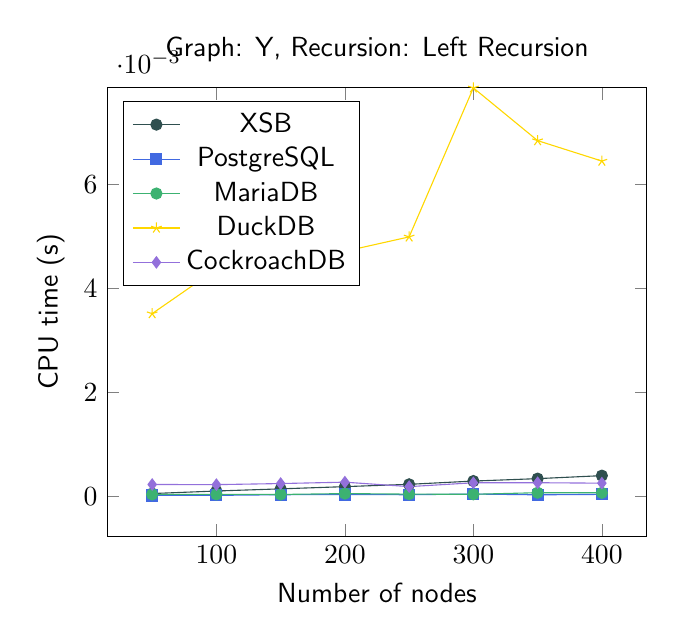
\begin{tikzpicture}
    \begin{axis}[
        title={Graph: Y, Recursion: Left Recursion},
        xlabel={Number of nodes},
        ylabel={CPU time (s)},
        legend pos={north west},
        ymax=0.007860800000000001
    ]
    \addplot+[DarkSlateGray, mark options={color=DarkSlateGray}] coordinates {(50,5.660000000000009e-05) (100,0.00010559999999999988) (150,0.0001469999999999996) (200,0.00018959999999999943) (250,0.0002341999999999996) (300,0.00029700000000000055) (350,0.0003436000000000002) (400,0.00040120000000000043)};
\addlegendentry{XSB}
\addplot+[RoyalBlue, mark options={color=RoyalBlue}] coordinates {(50,2.03999999999982e-05) (100,2.1800000000005148e-05) (150,3.3800000000006046e-05) (200,3.900000000000015e-05) (250,3.3800000000006046e-05) (300,4.7200000000002794e-05) (350,3.219999999999334e-05) (400,4.0399999999995995e-05)};
\addlegendentry{PostgreSQL}
\addplot+[MediumSeaGreen, mark options={color=MediumSeaGreen}] coordinates {(50,3.999999999998449e-05) (100,4.140000000001365e-05) (150,3.900000000000015e-05) (200,5.600000000001159e-05) (250,4.5400000000006545e-05) (300,4.2199999999992244e-05) (350,7.300000000000084e-05) (400,7.119999999999349e-05)};
\addlegendentry{MariaDB}
\addplot+[Gold, mark options={color=Gold}] coordinates {(50,0.003517999999999999) (100,0.0043744000000000005) (150,0.005438399999999999) (200,0.004716999999999994) (250,0.004993999999999976) (300,0.007860800000000001) (350,0.006845999999999996) (400,0.006453000000000009)};
\addlegendentry{DuckDB}
\addplot+[MediumPurple, mark options={color=MediumPurple}] coordinates {(50,0.00023079999999999767) (100,0.00022820000000001173) (150,0.0002489999999999992) (200,0.0002755999999999981) (250,0.00018999999999999017) (300,0.0002635999999999972) (350,0.0002650000000000041) (400,0.00025639999999997886)};
\addlegendentry{CockroachDB}

    \end{axis}
\end{tikzpicture}
\end{document}
